% Created 2024-10-16 śro 21:35
% Intended LaTeX compiler: pdflatex
\documentclass[../main.tex]{subfiles}

% \usepackage[a4paper, margin=3cm]{geometry}
% \usepackage{amssymb} // not working

\usepackage[T1]{fontenc}
\usepackage[utf8]{inputenc}
\usepackage{graphicx}
\usepackage{longtable}
\usepackage{wrapfig}
\usepackage{rotating}
\usepackage[normalem]{ulem}
\usepackage{amsmath}
\usepackage{capt-of}
\usepackage{hyperref}
\usepackage{siunitx}
\usepackage{float}
\usepackage[polish]{babel}

\graphicspath{{../}}
\author{Wojciech Paderewski}
\date{\today}
\title{testy}
\hypersetup{
 pdfauthor={Wojciech Paderewski},
 pdftitle={testy},
 pdfkeywords={},
 pdfsubject={},
 pdflang={Polish}}

\begin{document}
W tym rozdziale opisano testowanie poszczególnych 
modułów oraz całego układu, które pozwoliło na sprawdzenie poprawności działania oraz zidentyfikowanie błędów.

\subsection{Testy przetwornicy wysokiego napięcia}
Po napisaniu i wgraniu oprogramowania do mikrokontrolera, przystąpiono do testów przetwornicy wysokiego napięcia.
Sprawdzono działanie regulacji napięcia za pomocą potencjometru cyfrowego. Zakładany zakres napięcia wyjściowego to 130-220V.

W celu weryfikacji pomierzono zależność napięcia wyjściowego od podanej wartości na potencjometrze cyfrowym.

//tabela z wynikami pomiarów

\begin{table}[H]
    \centering
    \begin{tabular}{|c|c|}
        \hline
        Napięcie wyjściowe [V] & Wartość potencjometru cyfrowego \\
        \hline
        130 & 0 \\
        140 & 17 \\
        150 & 36 \\
        160 & 51 \\
        170 & 64 \\
        180 & 78 \\
        190 & 96 \\
        200 & 112 \\
        210 & 127 \\
        \hline
    \end{tabular}
    \caption{Zależność napięcia wyjściowego od wartości potencjometru cyfrowego}


\begin{figure}[H]
    \centering
    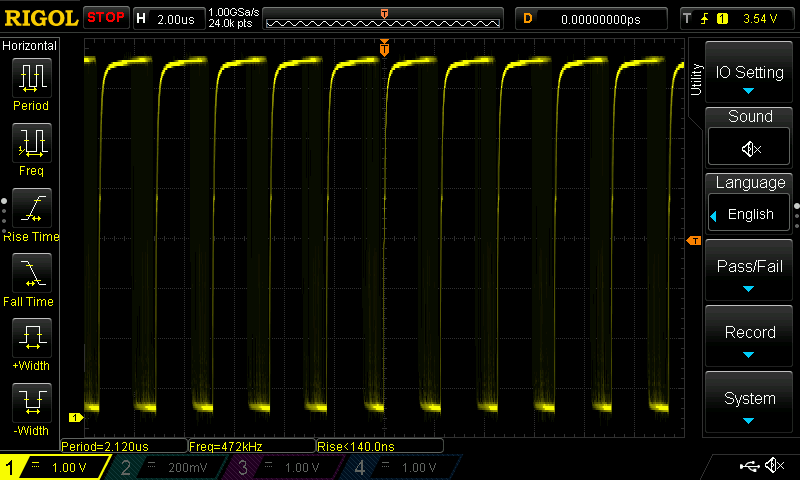
\includegraphics[width=1\textwidth]{duty_140.png}
    \caption{Wypełnienie sygnału sterującego przy napieciu wyjściowym 140V}
\end{figure}

\begin{figure}[H]
    \centering
    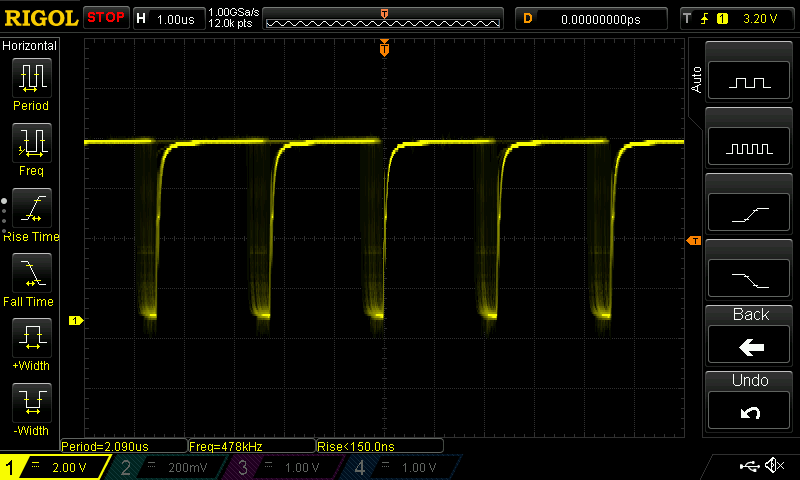
\includegraphics[width=1\textwidth]{duty_200.png}
    \caption{Wypełnienie sygnału sterującego przy napieciu wyjściowym 200V}
\end{figure}


\subsection{Pobór mocy}


\subsection{Testy całego układu}

\end{document}


